\chapter{Introduction}
\section{Strontium is boring}
\authorAmSa
Some introducing words \dots
Zitierungen:

ganz normal inline im Text mit Seitenangaben \cite[6]{franke17}

oder an den Text in Klammern angehangen, mit Seitenangaben und Kommentar \autocites(see also his earlier work)[347-348]{franke17}

\section{Motivation}
Give a general overview on the subject of this thesis! In which context shall the content of this thesis \index{Thesis} be seen? 

Nutze autoref\{label\} ohne vorher Abbildung , figure, table oder sonstiges zu nutzen, z.B. \autoref{fig:Kossmat} oder \autoref{tab:Laser} und \autoref{equ:Franke1} 

\section{Bor heilt}
Am Anfang eines Satzes sollte Autoref\{label\} genutzt werden. Das ergibt einene ausgeschribene Referenz.

\Autoref{equ:Franke1} zeigt die komplette Ausschreibung. Using $\pi$ is always advised.

Abkürzungen können im File AbbreviationDefinitions definiert werden und einfach über ac\{acronym\} abgerufen werden. Beim ersten Mal wird alles angezeigt: \ac{sundials} . Danach nur die Kurzform \ac{sundials}

\chapter{Regionalgeologie}

\section{Lithologie}
\authorAnGu
Der Hinweis auf den Author sollte nicht vor einer Überschrift stehen, sondern besser unmittelbar vor dem Text. Das Kartiergebiet befindet sich im Rheinischen Schiefergebirge. Dieses ist Teil der Mitteldeutschen variszischen Orogenese. Der Gebirgsbildung vorangestellt ist eine, noch nicht in allen Einzelheiten verstandene Beckenentwicklung, im Devon und Unterkarbon. \cite{franke17}

\Autoref{fig:Kossmat} nun übergeordneten Kontext schlossen sich während der Akkretion Laurussias und Gondwanas, das Rheiische und Rhenoherzynische Becken. Nach der Kossmat'schen Gliederung des deutschen Variszikums, befindet sich das Rheinische Schiefergebirge fast ausschließlich im Rhenoherzynikum, und wird südöstlich durch die nördliche Phyllitzone und das Mitteldeutsche Kritallinhoch begrenzt (siehe \autoref{fig:Kossmat}).

\begin{figure}[!htb]
\centering
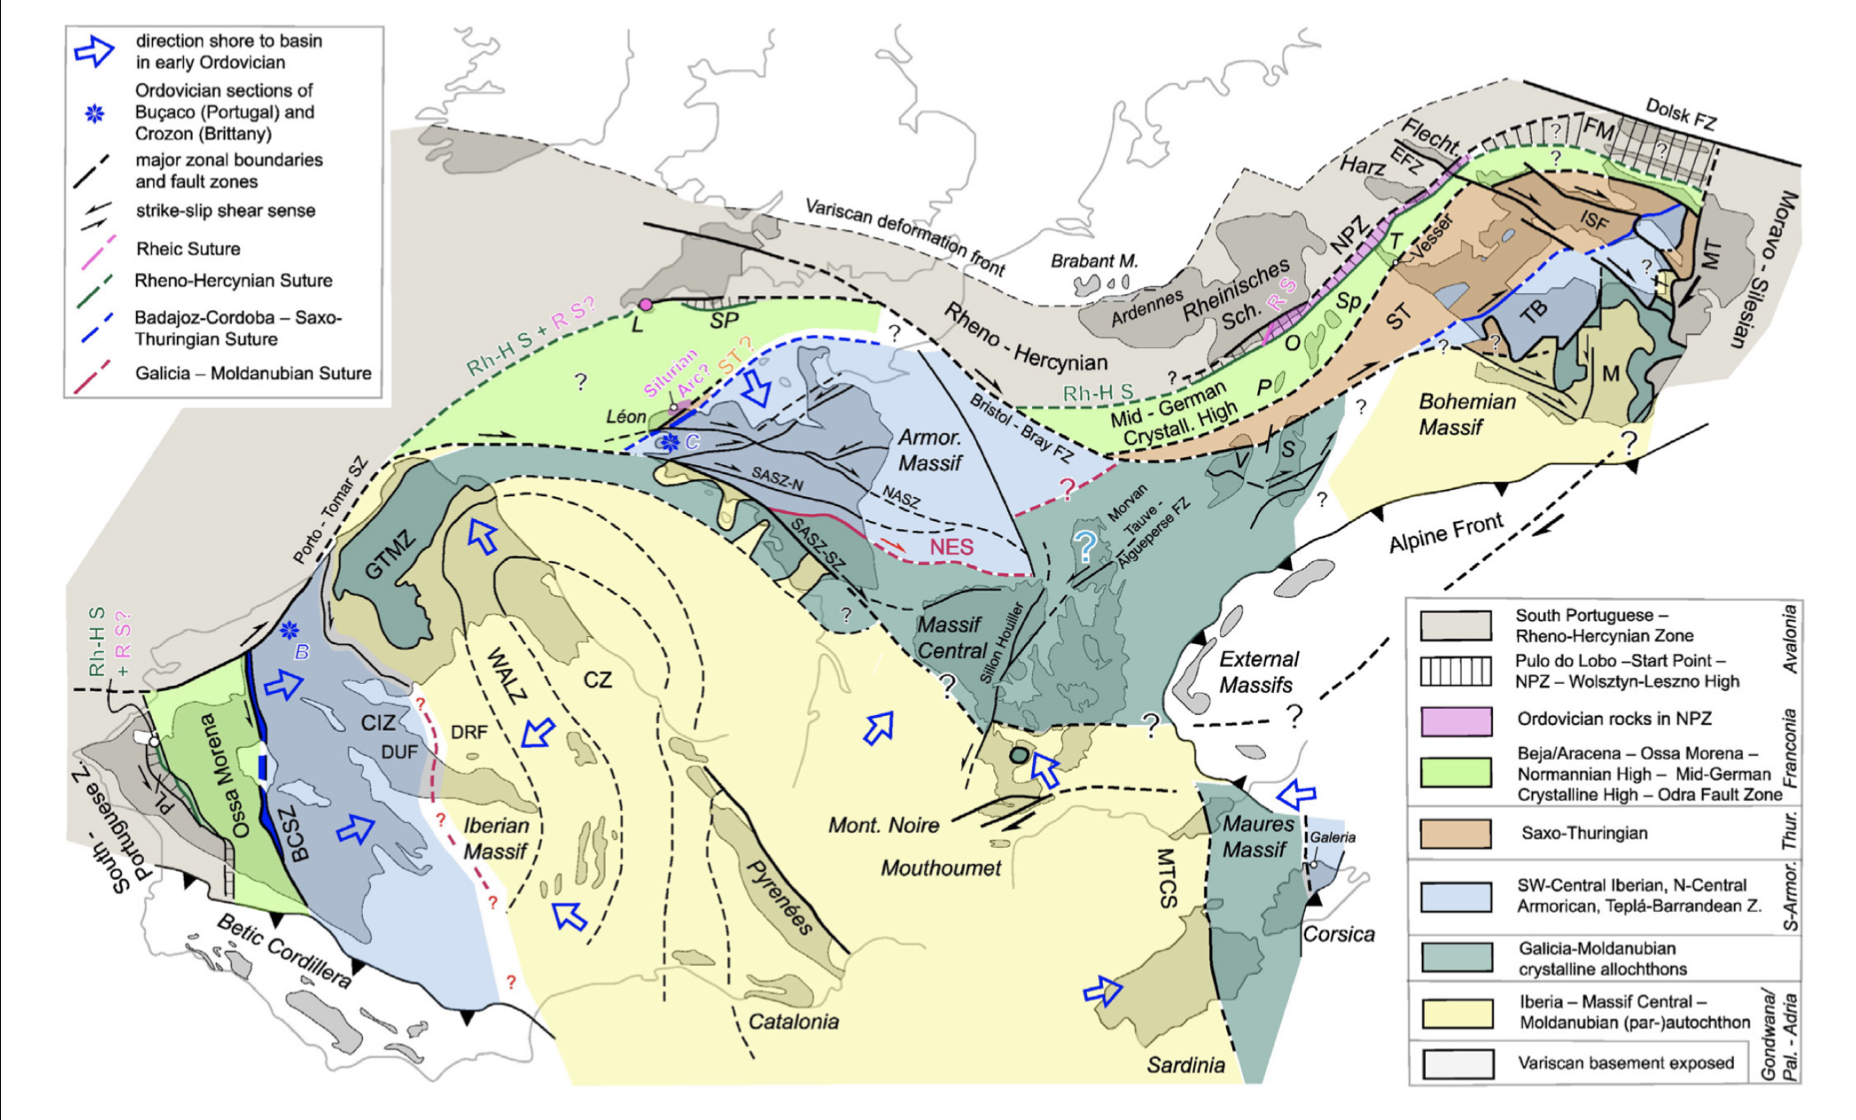
\includegraphics[width=\textwidth]{Ueberblick_Kossmat.png}
\caption{Europäisches Variszikum inklusive Rheinisches Schiefergebirge (\cite{franke17})}
\label{fig:Kossmat}
\end{figure} 

\subsection{Geometrische Geologie}
Aus den in \autoref{fig:Kossmat} dargestellten geometrischen Beziehungen folgt:

\begin{equation}
 sin(\alpha)=\frac{\Delta x_1}{\sqrt{(\Delta x_1)^2+s^2}}
 \label{equ:Franke1}
\end{equation}

\Autoref{tab:Laser} am Anfang und so weiter Im Unterdevon kam es zu Transgression und damit einhergehender Hungersedimentation, sowie anschließenden Flyscheintrag, in Folge, der im Südosten einsetzenden Gebirgsbildung. Kulm-Alaunschiefer, Kulm-Kieselschiefer, Kulmtonschiefer, und Kulm-Grauwacken belegen diese. Letztere sind im Kartiergebiet Arfeld jedoch nicht auffindbar. Die Nordwest-Südost gerichtete Einengung hatte intensive nordwest vergente Faltung, sowie Verkürzung der kontinentalen Kruste um 51 Prozent zur Folge. 

\begin{table}[!h]
\centering
\caption{Messwerte und Ergebnisse}
\label{tab:Laser}
\begin{tabular}{@{}llll@{}}
\toprule
{Messung} & {$\Delta x[cm]$} & {$s[cm]$} & {$\lambda[nm]$} \\ \midrule
rot     & 9,5           & 26    & 689          \\
grün    & 7,3         & 26    & 540          \\ \bottomrule
\end{tabular}
\end{table}



